

% Default to the notebook output style


% Inherit from the specified cell style.




    
\documentclass{article}

    
    
    \usepackage{graphicx} % Used to insert images
    \usepackage{adjustbox} % Used to constrain images to a maximum size 
    \usepackage{color} % Allow colors to be defined
    \usepackage{enumerate} % Needed for markdown enumerations to work
    \usepackage{geometry} % Used to adjust the document margins
    \usepackage{amsmath} % Equations
    \usepackage{amssymb} % Equations
    \usepackage[mathletters]{ucs} % Extended unicode (utf-8) support
    \usepackage[utf8x]{inputenc} % Allow utf-8 characters in the tex document
    \usepackage{fancyvrb} % verbatim replacement that allows latex
    \usepackage{grffile} % extends the file name processing of package graphics 
                         % to support a larger range 
    % The hyperref package gives us a pdf with properly built
    % internal navigation ('pdf bookmarks' for the table of contents,
    % internal cross-reference links, web links for URLs, etc.)
    \usepackage{hyperref}
    \usepackage{longtable} % longtable support required by pandoc >1.10
    

    
    \definecolor{orange}{cmyk}{0,0.4,0.8,0.2}
    \definecolor{darkorange}{rgb}{.71,0.21,0.01}
    \definecolor{darkgreen}{rgb}{.12,.54,.11}
    \definecolor{myteal}{rgb}{.26, .44, .56}
    \definecolor{gray}{gray}{0.45}
    \definecolor{lightgray}{gray}{.95}
    \definecolor{mediumgray}{gray}{.8}
    \definecolor{inputbackground}{rgb}{.95, .95, .85}
    \definecolor{outputbackground}{rgb}{.95, .95, .95}
    \definecolor{traceback}{rgb}{1, .95, .95}
    % ansi colors
    \definecolor{red}{rgb}{.6,0,0}
    \definecolor{green}{rgb}{0,.65,0}
    \definecolor{brown}{rgb}{0.6,0.6,0}
    \definecolor{blue}{rgb}{0,.145,.698}
    \definecolor{purple}{rgb}{.698,.145,.698}
    \definecolor{cyan}{rgb}{0,.698,.698}
    \definecolor{lightgray}{gray}{0.5}
    
    % bright ansi colors
    \definecolor{darkgray}{gray}{0.25}
    \definecolor{lightred}{rgb}{1.0,0.39,0.28}
    \definecolor{lightgreen}{rgb}{0.48,0.99,0.0}
    \definecolor{lightblue}{rgb}{0.53,0.81,0.92}
    \definecolor{lightpurple}{rgb}{0.87,0.63,0.87}
    \definecolor{lightcyan}{rgb}{0.5,1.0,0.83}
    
    % commands and environments needed by pandoc snippets
    % extracted from the output of `pandoc -s`
    \DefineVerbatimEnvironment{Highlighting}{Verbatim}{commandchars=\\\{\}}
    % Add ',fontsize=\small' for more characters per line
    \newenvironment{Shaded}{}{}
    \newcommand{\KeywordTok}[1]{\textcolor[rgb]{0.00,0.44,0.13}{\textbf{{#1}}}}
    \newcommand{\DataTypeTok}[1]{\textcolor[rgb]{0.56,0.13,0.00}{{#1}}}
    \newcommand{\DecValTok}[1]{\textcolor[rgb]{0.25,0.63,0.44}{{#1}}}
    \newcommand{\BaseNTok}[1]{\textcolor[rgb]{0.25,0.63,0.44}{{#1}}}
    \newcommand{\FloatTok}[1]{\textcolor[rgb]{0.25,0.63,0.44}{{#1}}}
    \newcommand{\CharTok}[1]{\textcolor[rgb]{0.25,0.44,0.63}{{#1}}}
    \newcommand{\StringTok}[1]{\textcolor[rgb]{0.25,0.44,0.63}{{#1}}}
    \newcommand{\CommentTok}[1]{\textcolor[rgb]{0.38,0.63,0.69}{\textit{{#1}}}}
    \newcommand{\OtherTok}[1]{\textcolor[rgb]{0.00,0.44,0.13}{{#1}}}
    \newcommand{\AlertTok}[1]{\textcolor[rgb]{1.00,0.00,0.00}{\textbf{{#1}}}}
    \newcommand{\FunctionTok}[1]{\textcolor[rgb]{0.02,0.16,0.49}{{#1}}}
    \newcommand{\RegionMarkerTok}[1]{{#1}}
    \newcommand{\ErrorTok}[1]{\textcolor[rgb]{1.00,0.00,0.00}{\textbf{{#1}}}}
    \newcommand{\NormalTok}[1]{{#1}}
    
    % Define a nice break command that doesn't care if a line doesn't already
    % exist.
    \def\br{\hspace*{\fill} \\* }
    % Math Jax compatability definitions
    \def\gt{>}
    \def\lt{<}
    % Document parameters
    \title{Filtros}
    
    
    

    
    % Prevent overflowing lines due to hard-to-break entities
    \sloppy 
    % Setup hyperref package
    \hypersetup{
      breaklinks=true,  % so long urls are correctly broken across lines
      colorlinks=true,
      urlcolor=blue,
      linkcolor=darkorange,
      citecolor=darkgreen,
      }
    % Slightly bigger margins than the latex defaults
    
    \geometry{verbose,tmargin=1in,bmargin=1in,lmargin=1in,rmargin=1in}
    
    

    \begin{document}
    
    
    \maketitle
    
    

    
    \section{Filtro}\label{filtro}

Un filtro eléctrico o filtro electrónico es un elemento que discrimina
una determinada frecuencia o gama de frecuencias de una señal eléctrica
que pasa a través de él, pudiendo modificar tanto su amplitud como su
fase

Con independencia de la realización concreta del filtro, salvo que debe
ser lineal, (analógico, digital o mecánico) su forma de comportarse se
describe por su función de transferencia. Ésta determina la forma en que
la señal aplicada cambia en amplitud y en fase, para cada frecuencia, al
atravesar el filtro. La función de transferencia elegida tipifica el
filtro.

\subsection{Antecedentes}\label{antecedentes}

En está sección se dan algunas definiciones necesarias para el manejo de
filtros.

\subsubsection{Función de
transferencía}\label{funciuxf3n-de-transferencuxeda}

Una función de transferencia es un modelo matemático que a través de un
cociente relaciona la respuesta de un sistema (modelada) a una señal de
entrada o excitación (también modelada). En la teoría de control, a
menudo se usan las funciones de transferencia para caracterizar las
relaciones de entrada y salida de componentes o de sistemas que se
describen mediante ecuaciones diferenciales lineales e invariantes en el
tiempo.

La función de trasferencia de un \emph{sistema lineal e invariante en el
tiempo (LTI)}, se define como el cociente entre la \emph{transformada de
Laplace} de la salida y la \emph{transformada de Laplace} de la entrada,
bajo la suposición de que las condiciones iniciales son nulas. De forma
general se representa por la expresión:


\begin{equation}
H (s) = \frac {Y(s)} {X(s)}
\end{equation}


donde $H (s)$ es la función de transferencia (también notada como
$G (s)$ ); $Y (s)$ es la transformada de Laplace de la respuesta y
$X (s)$ es la transformada de Laplace de la señal de entrada.

La función de transferencia también puede considerarse como la respuesta
de un sistema inicialmente inerte a un impulso como señal de entrada:


\begin{equation}
H(s) = \mathcal{L} \left \{ h(t) \right \} = \int_{0}^\infty e^{-st} h(t)\,dt 
\end{equation}


Es importante señalar que un impulso de entrada normalmente se
representa con la función \emph{Delta de Dirac}, está señal ideal
permite modelar un sistema ya que su \emph{Transformada de Fourier}
incluye infinitos componentes de frecuencia. Por lo que, se dice que un
impulso a la entrada de un sistema permite obtener la respuesta del
sistema a todas las frecuencias. Sin embargo, un impulso no es
\textbf{Realizable en la practica} porque implicaría tener un sistema
que puede producir todas las frecuencias en instante con duración 0, lo
cual implicaria un sistema con infinita energía.

\subsubsection{Diagrama de Bode}\label{diagrama-de-bode}

Un Diagrama de Bode es una representación gráfica que sirve para
caracterizar la respuesta en frecuencia de un sistema. Normalmente
consta de dos gráficas separadas, una que corresponde con la magnitud de
dicha función y otra que corresponde con la fase. Recibe su nombre del
científico senegalés que lo desarrolló, Hendrik Wade Bode.

Es una herramienta muy utilizada en el análisis de circuitos en
electrónica, siendo fundamental para el diseño y análisis de filtros y
amplificadores. De forma analitica, el diagrama de bode se obitene de la
función de transferencia, la cual es una función compleja ya que
$s=\sigma+j\omega$.

\emph{El diagrama de magnitud de Bode} dibuja el módulo de la función de
transferencia (ganancia) en decibelios en función de la frecuencia (o la
frecuencia angular) en escala logarítmica. Se suele emplear en procesado
de señal para mostrar la respuesta en frecuencia de un sistema lineal e
invariante en el tiempo.

\emph{El diagrama de fase de Bode} representa la fase de la función de
transferencia en función de la frecuencia (o frecuencia angular) en
escala logarítmica. Se puede dar en grados o en radianes. Permite
evaluar el desplazamiento en fase de una señal a la salida del sistema
respecto a la entrada para una frecuencia determinada. En sistemas
eléctricos esta fase deberá estar acotada entre -90° y 90°.

El diagrama de bode permite de forma rapida análisar el comportamiento
de un sistema ante entradas con difrentes frecuencias. Por ejemplo,
tenemos una señal $A\sin(\omega t)$ a la entrada del sistema y asumimos
que el sistema atenúa por un factor $x$ y desplaza en fase $−\theta$. En
este caso, la salida del sistema será $(A/x) \sin(\omega t − \theta)$.
Generalmente, este desfase es función de la frecuencia y representa un
retraso en tiempo, lo cual indica que el tiempo que toma a una señal de
entrada $x$ verse reflejada en la salida $y$ depende de la frecuencia de
la señal de entrada; esta dependencia es lo que nos muestra el Bode.

\textbf{Transformada de Laplace} La transformada de Laplace de una
función $f(t)$ definida (en ecuaciones diferenciales, o en análisis
matemático o en análisis funcional) para todos los números positivos
$t \geq 0$, es la función $F(s)$, definida por: \[
F(s) = \mathcal{L} \left\{f(t)\right\} =\int_{0}^\infty e^{-st} f(t)\,dt.
\] siempre y cuando la integral esté definida. \#\#Tipos de Filtros

\subsubsection{Filtro paso bajo}\label{filtro-paso-bajo}

Un filtro paso bajo corresponde a un filtro caracterizado por permitir
el paso de las frecuencias más bajas y atenuar las frecuencias más
altas. El filtro requiere de dos terminales de entrada y dos de salida,
de una caja negra, también denominada cuadripolo o bipuerto, así todas
las frecuencias se pueden presentar a la entrada, pero a la salida solo
estarán presentes las que permita pasar el filtro. De la teoría se
obtiene que los filtros están caracterizados por sus funciones de
transferencia, así cualquier configuración de elementos activos o
pasivos que consigan cierta función de transferencia serán considerados
un filtro de cierto tipo.

En particular la función de transferencia de un filtro pasa bajo de
primer orden corresponde a

\begin{equation}\label{eq:lpf1o}
H(s)=k\frac{1}{1+\frac{s}{\omega_c}} \,
\end{equation}

donde la constante $k \,$ es sólo una ponderación correspondiente a la
ganancia del filtro. En la función de transferencia anterior
$\omega_c \,$ corresponde a la frecuencia de corte propia del filtro,
aquel valor de frecuencia para el cual la amplitud de la señal de
entrada se atenúa 3 dB.

Una tecnica de análisis es proponer funciónes de transferencia prototipo
donde $\omega_{c}=1$ y $K=1$, aplicandolo a \eqref{eq:lpf1o}, se tiene
que la función prototipo para un filtro paso bajo de primer orden es:

\begin{equation}\label{eq:lpf1op}
H(s)=\frac{1}{s+1}
\end{equation}

luego posteriormente se rescala el filtro considerando una nueva
variable

\[
p=\frac{s}{a}
\]

donde $s$ es la variable de Laplace de la función prototipo, $a$ es el
parámetro de rescalamiento y $p$ es la variable de Laplace de la función
del filtro reescalado.

\[
H(p)=G(P)|_{p=s/a}=G(s/a)
\]


    \begin{center}
    \adjustimage{max size={0.9\linewidth}{0.9\paperheight}}{Filtros_files/Filtros_1_0.png}
    \end{center}
    { \hspace*{\fill} \\}
    
    De forma análoga al caso de primer orden, los filtros de pasa bajo de
mayor orden también se caracterízan por su función de transferencia, por
ejemplo la función de transferencia de un filtro paso bajo de segundo
orden corresponde a

\begin{equation}
H(s) =K \frac{\omega_0^{2}}{  s^{2} + 2 \alpha s + \omega_{0}^{2} } 
\end{equation}

donde $\omega_0$ es la frecuencia natural de resonancia (en radianes),
$\alpha$ es la atenuación del sistema y se relación con el coefciente de
amortiguamiento $\xi$ y el factor de calidad $Q$ a través de la
expresión:

\begin{equation}
2\alpha=2\omega_{o} \xi=\frac{\omega_{o}}{Q}
\end{equation}

Es importante recordar que un para obtener un filtro Butterworth
máximamente planar se requiere que $Q=1/\sqrt{2}$. El factor de calidad
$Q$ es un parámetro que mide la relación entre la energía reactiva que
almacena y la energía que disipa durante un ciclo completo de la señal.
Un alto factor $Q$ indica una tasa baja de pérdida de energía en
relación a la energía almacenada por el resonador.

\begin{equation}
H(s) = \frac{1}{  s^{2} + \frac{1}{Q} s + 1 } 
\end{equation}


    \begin{center}
    \adjustimage{max size={0.9\linewidth}{0.9\paperheight}}{Filtros_files/Filtros_3_0.png}
    \end{center}
    { \hspace*{\fill} \\}
    
    \subsubsection{Filtro Paso Alto}\label{filtro-paso-alto}

Un filtro paso alto (HPF) es un tipo de filtro electrónico en cuya
respuesta en frecuencia se atenúan las componentes de baja frecuencia
pero no las de alta frecuencia, éstas incluso pueden amplificarse en los
filtros activos. La alta o baja frecuencia es un término relativo que
dependerá del diseño y de la aplicación.

\subsection{Filtros de segundo orden}\label{filtros-de-segundo-orden}

\subsubsection{Filtro Sallem-Key}\label{filtro-sallem-key}

\begin{figure}[htbp]
\centering
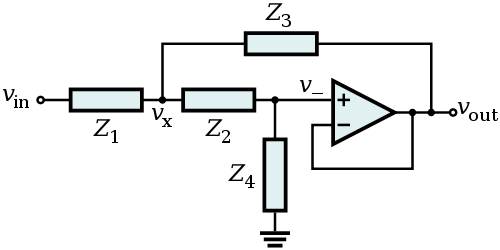
\includegraphics{images/sallemkeyideal.png}
\caption{Sallem-Key}
\end{figure}

    La estructura general del filtro salem-key se muestra en la figura
Considerando que el OPAM es ideal, entonces se tiene que:

\begin{eqnarray}
 V_{-}=V_{+}&=V_{out} \label{eq:opamv} \\
 i_{-}=i_{+}&=0 \label{eq:opami}
 \end{eqnarray}

Si cosideramos la ley de krichoff de Nodos y la ley de Ohm en el nodo de
$V_{x}$ se tiene que:

\begin{equation}\label{eq:vx}
\frac{v_{\text{in}}-v_x}{Z_1}=\frac{v_x-v_{\text{out}}}{Z_3}+\frac{v_x-v_-}{Z_2}
\end{equation}

Mientras que en el nodo $V_{+}$ si se considera \eqref{eq:opamv}, se
tiene que:

\begin{equation}
\frac{v_x-v_{\text{out}}}{Z_2}=\frac{v_{\text{out}}}{Z_4},
\end{equation}

despejando $V_{x}$

\begin{equation}\label{eq:vxvout}
v_x=v_{\text{out}} \left( \frac{Z_2}{Z_4}+1 \right).
\end{equation}

Si consideramos las expresiones \eqref{eq:opamv}, \eqref{eq:vx} y
\eqref{eq:vxvout} se tiene que la función de transferencia

\begin{equation}\label{eq:transsallemkey}
\frac{v_{\text{out}}}{v_{\text{in}}} = \frac{Z_3 Z_4}{Z_1 Z_2 + Z_3(Z_1 + Z_2) + Z_3 Z_4}
\end{equation}

    \subsubsection{Filtro pasabajas}\label{filtro-pasabajas}

En el caso de la celda de Sallem-Key para construir un filtro paso bajas
es necesario que:

\[
Z_1 = R_1, \quad Z_2 = R_2, \quad Z_3 = \frac{1}{s C_1}, \quad \text{y} \quad Z_4 = \frac{1}{s C_2}.\, 
\]

\begin{figure}[htbp]
\centering
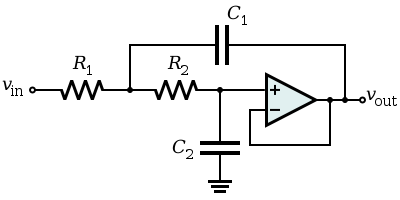
\includegraphics{images/sallemkey.png}
\caption{Sallem-Key LPF}
\end{figure}

por lo que la función de transferencia \eqref{eq:transsallemkey} queda
expresada como:


    \begin{Verbatim}[commandchars=\\\{\}]
\textbackslash{}frac\{1\}\{C\_\{1\} C\_\{2\} R\_\{1\} R\_\{2\} s\^{}\{2\} + C\_\{2\} s \textbackslash{}left(R\_\{1\} + R\_\{2\}\textbackslash{}right) + 1\}
    \end{Verbatim}

    \begin{equation}\label{eq:sallemkeybaja}
\frac{1}{C_{1} C_{2} R_{1} R_{2} s^{2} +  s C_{2} \left(R_{1} + R_{2}\right) + 1}
\end{equation}

    de la expresión \eqref{eq:sallemkeybaja} tenemos que:

\begin{equation}\label{eq:sallemkeywo}
\omega_{o}=\frac{1}{\sqrt{C_{1} C_{2} R_{1} R_{2}}}
\end{equation}

y

\begin{equation}\label{eq:sallemkeyq}
Q = { \omega_0 \over 2 \alpha } = \frac{ \sqrt{ R_1 R_2 C_1 C_2 } }{ C_2 \left( R_1 + R_2 \right) } 
\end{equation}

    de las expresiones \eqref{eq:sallemkeywo} y \eqref{eq:sallemkeyq}, se
tiene que multiples valores de $C_{1},C_{2},R_{1},R_{2}$ permiten
obtener la misma frecuencia $\omega_{o}$ y $Q$.

Una tecnica común es considerar que

\[
R_{1}=R_{2},C_{1}=C_{2}
\]

por lo que se tiene que las expresiones \eqref{eq:sallemkeywo} y
\eqref{eq:sallemkeyq} se reducen a

\[
\omega_{o}=\frac{1}{RC}
\]

y

\[
Q=\frac{1}{2}
\]

    \subsubsection{Ejemplo}\label{ejemplo}

Si consideramos un filtro pasabajas con una frecuencia de corte de
$f_{o}=15KHz$.

Si proponemos que $C=1nF$, entonces de la expresión
\eqref{eq:sallemkeywo}, se tiene que

\[
R=\frac{1}{2\pi f_{o} C}
\]


    
    
        \begin{equation*}
        10610.32953945969
        \end{equation*}

    

    sustituyendo valores se tiene que: \[
R=10.610k\Omega
\] Considerando que la función de transferencia del filtro se puede
representar como:

\begin{equation}
H=\frac{1}{b_{0}s^{2}+b_{1}s+b_{2}}
\end{equation}

donde


    \begin{Verbatim}[commandchars=\\\{\}]
\textbackslash{}begin\{bmatrix\}1.1257909293593088e-10, \& 2.122065907891938e-05, \& 1\textbackslash{}end\{bmatrix\}
    \end{Verbatim}
$
    \begin{bmatrix}b_{0}=1.1257909293593088\times10^{-10}, & b_{1}=2.122065907891938\times10^{-05}, & b_{2}=1\end{bmatrix}
$
Si se obtiene la gráfica de bode del sistema se tiene que la respuesta
del filtros es


    \begin{center}
    \adjustimage{max size={0.9\linewidth}{0.9\paperheight}}{Filtros_files/Filtros_16_0.png}
    \end{center}
    { \hspace*{\fill} \\}
    


    \begin{center}
    \adjustimage{max size={0.9\linewidth}{0.9\paperheight}}{Filtros_files/Filtros_18_0.png}
    \end{center}
    { \hspace*{\fill} \\}
    
    $R_1=mR,\,R_2=R,\,C_1=nC,\,C_2=C.\, $

Therefore, the f\_0, and Q, expressions are \[
\omega_0 = 2 \pi f_0 = \frac{1}{RC\sqrt{mn}},\, 
\] and \[
Q = \frac{\sqrt{mn}}{m+1}. 
\]

    \subsection{Filtro Rauch}\label{filtro-rauch}

Filtro de segundo orden con un solo apmplificador operacional su
estructura es

\begin{figure}[htbp]
\centering
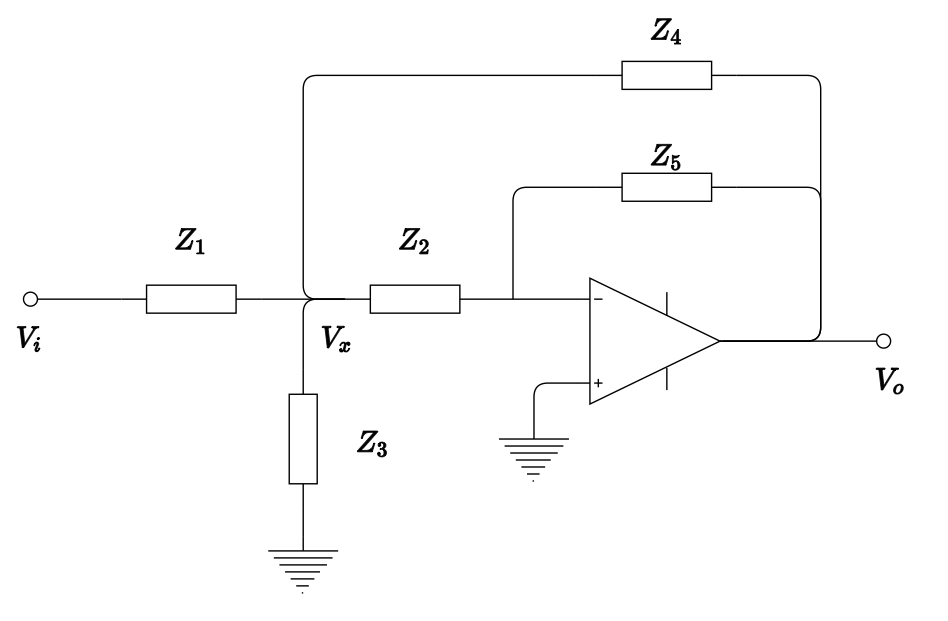
\includegraphics{images/filter_rauch.png}
\caption{Filtro Rauch}
\end{figure}

en el nodo de $V_{x}$ aplicando la ley de krichof de nodos se tiene que

\begin{equation}\label{eq:vxrauch}
\frac{V_{x}}{Z_{2}}+\frac{V_{x}}{Z_{3}}-\frac{V_{i}-V_{x}}{Z_{1}}-\frac{V_{o}-V_{x}}{Z_{4}}=0
\end{equation}

si se considera que idealmente la corriente en la entrada del opam es 0,
entonces en $V_{-}$ se tiene que:

\begin{equation}\label{eq:v-rauch}
i_{Z2}=-i_{Z5}
\end{equation}

por lo que se tiene que:

\begin{equation}
V_{x}=-\frac{V_{o}Z_{2}}{Z_{5}}
\end{equation}

sustituyendo en \eqref{eq:vxrauch}


    \begin{Verbatim}[commandchars=\\\{\}]
- \textbackslash{}frac\{Vo Z\_\{2\}\}\{Z\_\{3\} Z\_\{5\}\} - \textbackslash{}frac\{Vo\}\{Z\_\{5\}\} - \textbackslash{}frac\{1\}\{Z\_\{4\}\} \textbackslash{}left(\textbackslash{}frac\{Vo Z\_\{2\}\}\{Z\_\{5\}\} + Vo\textbackslash{}right) - \textbackslash{}frac\{1\}\{Z\_\{1\}\} \textbackslash{}left(Vi + \textbackslash{}frac\{Vo Z\_\{2\}\}\{Z\_\{5\}\}\textbackslash{}right)
    \end{Verbatim}

    \[
- \frac{Vo Z_{2}}{Z_{3} Z_{5}} - \frac{Vo}{Z_{5}} - \frac{1}{Z_{4}} \left(\frac{Vo Z_{2}}{Z_{5}} + Vo\right) - \frac{1}{Z_{1}} \left(Vi + \frac{Vo Z_{2}}{Z_{5}}\right)=0
\]

despejando $V_{o}/V_{i}$ se tiene


    
    
    \begin{verbatim}
'- \\frac{Z_{3} Z_{4} Z_{5}}{Z_{1} Z_{2} Z_{3} + Z_{1} Z_{2} Z_{4} + Z_{1} Z_{3} Z_{4} + Z_{1} Z_{3} Z_{5} + Z_{2} Z_{3} Z_{4}}'
    \end{verbatim}

    

    \begin{equation}\label{eq:rauchtf}
\frac{V_{o}}{V_{i}}=\frac{-Z_{3} Z_{4} Z_{5}}{Z_{1} Z_{2} Z_{3} + Z_{1} Z_{2} Z_{4} + Z_{1} Z_{3} Z_{4} + Z_{1} Z_{3} Z_{5} + Z_{2} Z_{3} Z_{4}}
\end{equation}



    
    
        \begin{equation*}
        - \frac{R_{3}}{C_{1} C_{2} R_{1} R_{2} R_{3} s^{2} + C_{2} R_{1} R_{2} s + C_{2} R_{1} R_{3} s + C_{2} R_{2} R_{3} s + R_{1}}
        \end{equation*}

    


    
    
        \begin{equation*}
        - \frac{R_{3}}{C_{1} C_{2} R_{1} R_{2} R_{3} s^{2} + C_{2} s \left(R_{1} R_{2} + R_{1} R_{3} + R_{2} R_{3}\right) + R_{1}}
        \end{equation*}

    


    
    
        \begin{equation*}
        \frac{1}{C_{1} C_{2} R_{1} R_{2} s^{2} + \frac{C_{2} R_{1}}{R_{3}} R_{2} s + C_{2} R_{1} s + C_{2} R_{2} s + \frac{R_{1}}{R_{3}}}
        \end{equation*}

    


    
    
        \begin{equation*}
        \frac{1}{C_{1} C_{2} R_{2} R_{3}}
        \end{equation*}

    


    
    
        \begin{equation*}
        \frac{Z_{3} Z_{4} Z_{5}}{Z_{1} Z_{2} Z_{3} + Z_{1} Z_{2} Z_{4} + Z_{1} Z_{3} Z_{4} + Z_{1} Z_{3} Z_{5} + Z_{2} Z_{3} Z_{4}}
        \end{equation*}

    



    % Add a bibliography block to the postdoc
    
    
    
    \end{document}
